\chapter{Improvements to MAUT Based Generation of Compound Critiques}
\label{chap:modifications}
\section{Limitations of MAUT Based Critiquing:}
\label{sec:limitations}

We have seen in Sections \ref{sec:offline} and \ref{sec:liveUser} that MAUT based recommendation performs slightly better than Apriori algorithm in offline experiments and live user studies.
The reason for the improved performance of MAUT based recommendation is that compound critiques are generated through utilities given by MAUT and these critiques tend to be more relevant to the user than the ones generated by Apriori algorithm.
However, there are several limitations to MAUT based recommendation. Some of the limitations which we have addressed in this project are given below:
\begin{itemize}
\setlength{\itemsep}{5pt}
\item Critique strings in a given iteration can be very similar to each other. Hence it limits the number of different options that users have.
\item Preference model is updated only based on the most recently selected critique string. History of products/critique strings selected by the user is not considered while updating the preference model.
\item Top five products shown in the first cycle is same for all recommendation sessions irrespective of the user query.
\item In a particular recommendation cycle, if all the critique strings have "Higher Price", user is forced to select a critique string with "Higher Price". We would ideally not want to update the weight of the attribute $price$, since we cannot infer whether user is willing to compromise on $price$ attribute. But MAUT based recommendation algorithm will actually decrease the weight of $price$ attribute by a factor of $\beta$, thus promoting higher priced cameras in the next cycle.
%\item As an extension to the above point, Consider the case when there are 4 critique strings with "Lower Resolution" and 1 critique string with "Higher Resolution". If the user selects the critique string that has "Higher Resolution", we can update  the weight of 'Resolution' attribute by a higher factor.
\item The fact that a particular product has been preferred over the remaining (k-1) rejected products is not exploited when updating the preference model.

\end{itemize}
%put section numbers when all the description is done...
We address each of the above limitations and also propose some additional improvements to MAUT based recommendation in Sections \ref{sec:div} to \ref{sec:additive}.


\section{Diversity in Critiques}

A variant of \textit{\textbf{Bounded Greedy Selection}} algorithm described in \cite{boundedGreedy} was used to generate diverse critiques in every cycle.
The function \textit{GenCritiqueItems(PM, IS)} is modified as follows:\\
\\

\begin{algorithm}[ht]
  \SetKwInOut{Input}{input}\SetKwInOut{Output}{output}
  \DontPrintSemicolon
  %\Input{$PM$, $IS$}

  $R \gets \{\}$\\
  $CB' \gets IS$\\
  \For{ $i\gets0$ \KwTo $k$ }{
    Sort $CB'$ by $Quality(i, R, PM)$ for each case in IS; \\
    $R \gets R + First(CB')$;\\
    $CB' \gets CB' - First(CB')$;\\
  }
  \Return R
  \caption{GenCritiqueItems(PM, IS)}
  \label{algo:div}
\end{algorithm}

\begin{algorithm}[ht]
  \SetKwInOut{Input}{input}\SetKwInOut{Output}{output}
  \DontPrintSemicolon
  %\Input{$i$, $R$, $PM$}

  \If {$R == \{\}$} {return 0;}
  \Else {
      $retVal \gets \alpha \times utility(i, PM)$; \\
      $disSim \gets \frac{\sum_{r_j \in R} (1-critiqueSim(i,r_j))}{|R|}$;\\
      $retVal += (1-\alpha) \times disSim$;\\
      $return retVal$;\\
  }
  \Return retVal
  \caption{Quality(i, R, PM)}
  \label{algo:quality}
\end{algorithm}

$critiqueSim(a, b)$ returns the extent of overlap between the individual attribute directions of products $a$ and $b$.
We get the best results when $\alpha = 0.5$.
Introducing diverse critiques in every cycle results in significant improvement in the number of interaction cycles and it also improves user experience (Users don't prefer critiques being very similar to each other).


\begin{figure}
\centering
\begin{minipage}{.45\textwidth}
  \centering
  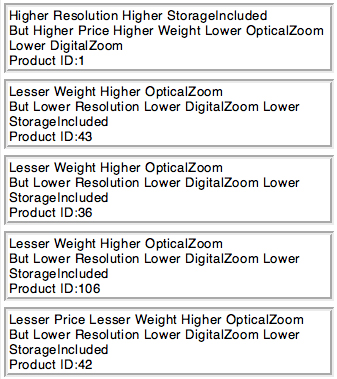
\includegraphics[width=1\linewidth]{figures-bharath/diversity1.jpg}
  \caption{Before diversifying critique strings}
  \label{fig:beforeDiv}
\end{minipage}%
\;\;\;\;\;\;
\begin{minipage}{.45\textwidth}
  \centering
  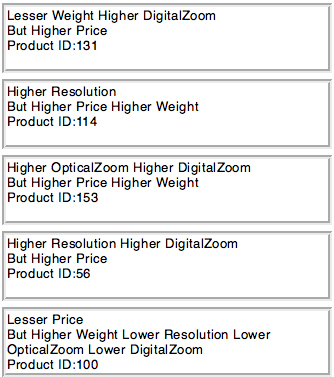
\includegraphics[width=1\linewidth]{figures-bharath/diversity2.jpg}
  \caption{After diversification}
  \label{fig:afterDiv}
\end{minipage}
\end{figure}


\section{Varying the level of diversity}
\label{sec:div2}
In Section \ref{sec:div}, we have discussed a method of introducing diversity in every cycle.
We know that, at the beginning of a recommendation session, an average user does not have a good understanding of the product space and trade-offs that exist between different product attributes.
But after interacting with the recommender system for a few cycles, he develops a good understanding of the product space and his preferences become more stable.
Therefore, it is a good idea to introduce diversity in the beginning of a recommendation session so that user will develop a better understanding of the product space and then show targeted recommendations after a few cycles when his preferences have stabilized.

We propose a new approach where diversity is varied adaptively according to whether user's preferences have stabilized.
Consider an attribute 'Price'.
If the maximum difference between prices of previous $K$(=3) products selected by the user is less than a pre-defined threshold, we assume that the user is satisfied with this particular product price and we promote cases that have a price closer to the average price of the $K$ products in the next cycle.
%Consdiering camera dataset, if the difference between 'weight' of each of the previous $K$(=3) selected products is less than a certain threshold,
If the maximum difference between the weights of the previous $K$(=3) products is greater than the pre-defined threshold, we assume that user's preference for the 'weight' attribute has not stabilized yet. 
Hence, we try to display products that are diverse to each other in terms of 'weight' attribute.
The numeric attributes for which we assume that user's preference has stabilized are classified into the set $simA$.
The other numeric attributes are classified into the set $divA$.
In the implementation, the function \textit{GenCritiqueItems(PM, IS)} is the same as described in Algorithm \ref{algo:div}.
The function \textit{Quality(p, R, PM)} is modified as follows:

\begin{algorithm}[ht]
  \SetKwInOut{Input}{input}\SetKwInOut{Output}{output}
  \DontPrintSemicolon
  %\Input{$i$, $R$, $PM$}

  $ret \gets \alpha \times utility(i, PM)$; \\
  $simA, divA$ = classifyAttributes(); \\
  $avg$ = previousKProductAttributeAverages(); \\
  $tmp \gets 0$;\\
  \For{ each attribute $x_i$ in $simA$ }{
      $tmp$ += (sim($avg(x_i)$, $p(x_i)$));\\
  }
  \For{ each attribute $x_i$ in $divA$ }{
      $tmp += \frac{\sum_{r_j \in R} (1-sim(p(x_i),r_j(x_i)))}{|R|}$;\\
  }

  $tmp = (1-\alpha) \times \frac{tmp} {\lvert simA\rvert + \lvert divA\rvert}$\\
  \Return $ret + tmp$ ;\\
  \caption{Quality(p, R, PM)}
  \label{algo:quality2}
\end{algorithm}

We will refer to the algorithm described in this section as \textbf{DIV2} in the subsequent sections.

\section{Additional preference to products that are similar to the most recent user selected product}
In addition to updating weights of numeric attributes and value functions of nominal attributes, we give an additional preference to the products that have a similar critique pattern as that of the most recently selected product.
The method of computing critique patterns for products has been discussed in Section \ref{sec:genCritique}.
The intuition behind this modification is that, if the user selects the critique string "Lower Price, Higher Resolution but Higher Weight", he is interested in those products where this trade-off is obeyed.
Considering only three attributes, Price, Resolution and Weight, if the critique pattern of the selected product is \{Price:$<$, Resolution:$>$, Weight:$>$\} and the critique pattern of a product $p$ in the case base is \{Price:$<$, Resolution:$>$, Weight:$<$\}, the overlap between the two critique patterns is 2/3.
The function $CalcUtility(PM, u)$ (Algorithm \ref{algo:utility}), which is used to calculate utility of products at the beginning of each cycle is modified as follows:

\begin{algorithm}[ht]
  \SetKwInOut{Input}{input}\SetKwInOut{Output}{output}
  \DontPrintSemicolon
  %\Input{$PM$, $IS$}

  retVal $\gets 0$;\\
  \For{ each attribute $x_i$ in $u$ }{
      retVal += $pw_i \times V(x_i)$
  }
  $p1 \gets $CritiquePattern(u);\\
  $p2 \gets $CritiquePattern(previousSelectedProduct);\\
  retVal += $overlap(p1, p2)$;\\
  \Return retVal
  \caption{CalcUtility(PM, u)}
  \label{algo:addPref}
\end{algorithm}



%\subsection{Generalization of the above where you can have multiple products}
In Algorithm \ref{algo:addPref}, we have considered the critique overlap between a product in the case-base and the product that is most recently selected by the user.
We now extend the above algorithm by considering the critique overlap of a product with all the products that have been selected so far.
The additional term added to the utility of a product,\textit{overlapTerm} is calculated as follows:
\begin{equation}
\label{eq:addPref}
addTerm(p) = \frac{\sum_{i=1}^{n} {w_i \times overlap(p,sel_i)}} {\sum_{i=1}^{n}w_i}
\end{equation}
In Equation \ref{eq:addPref}, $sel_i$ refers to the product selected by the user in $i^{th}$ cycle.
$w_i$ is the weight/importance associated with the overlap between the product $p$ and product selected in $i^{th}$ cycle.
In our implementation, we set $w_i = \frac{1}{2^{n-i}}$.
The modified \textit{CalcUtility(PM, u)} function is as follows:

\begin{algorithm}[ht]
  \SetKwInOut{Input}{input}\SetKwInOut{Output}{output}
  \DontPrintSemicolon
  %\Input{$PM$, $IS$}

  retVal $\gets 0$;\\
  \For{ each attribute $x_i$ in $u$ }{
      retVal += $pw_i \times V(x_i)$
  }
  \For { each product $t_i$ in previouslySelectedProducts} {
      $p1 \gets $CritiquePattern($u$);\\
      $p2 \gets $CritiquePattern($t_i$);\\
      retVal += $w_i \times overlap(p1, p2)$;\\
  }
  \Return retVal
  \caption{CalcUtility(PM, u)}
  \label{algo:addPref2}
\end{algorithm}

\section{Similar Products in the First Cycle}
As seen in Section \ref{sec:maut}, weights of numeric attributes and the value functions of nominal attributes are initialized to default values.
Therefore, the top $K$ utility products presented to the user in the first cycle is the same irrespective of initial preferences given by the user.
Instead of presenting the top $K$ utility products in the first cycle, we present products that are most similar to the user's query.
When the user selects one of those similar products, the preference model is updated in the proper direction such that the target product shows up quickly in top $K$ products.
%put pseudo-code of the function that has been modified...

\section{Selectively updating the weights of numeric attributes}
As seen in Section \ref{sec:maut}, the weight of a numeric attribute is either multiplied or divided by a constant factor $\beta (=2.0)$ depending on whether the new preference value is better than the old preference value or not.
But this approach has some limitations as discussed in Section \ref{sec:limitations}.
In a particular recommendation cycle, if all the critique strings have "Higher Price" as their sub-critique, the user is forced to select a critique string with "Higher Price".
The MAUT based recommendation algorithm will decrease the weight of $price$ attribute by a factor of $\beta$ and the algorithm will thus promote higher priced products in the next cycle.
We modify the implementation of MAUT based recommendation algorithm such that the weight of the $price$ attribute in such cases is not changed.
As an extension to the above limitation, if we consider the case when there are four critique strings with "Lower Resolution" and one critique string with "Higher Resolution". 
If the user selects critique string that has "Higher Resolution", we can infer that the user has strong preference for cameras with higher resolution and hence multiply the weight of the attribute 'resolution' by a higher factor.

%Put table here...

\section{Selectively updating value functions of nominal attributes}
As seen in Section \ref{sec:valueFunc}, the value of $\gamma$ used to update the value functions of nominal attributes is constant in each cycle.
Instead, we propose an alternative approach in which the value of $\gamma$ varies according to the number of alternatives the user rejected while choosing a particular attribute value. 
Stronger the preference the user has for a particular attribute value, higher is the value of $\gamma$.
The intuition for varying the value of $\gamma$ is as follows: Consider the case when there are five PCs displayed to the user and the manufacturers of the five PCs are "Compaq", "HP", "Apple", "Dell" and "Toshiba".
If the user selects the PC with "Compaq" as the manufacturer, we can see that he has accepted "Compaq" and rejected four other manufacturers.
Thus, we can say that the user has a strong preference for "Compaq" PCs.
On the other hand, in the case when all the five PCs have a screen size of 15 inches and the user selects the PC with screen-size of 15 inches, we cannot really infer whether the user has a strong preference for 15 inch PCs.
Generalizing the examples above, if $k$ is the value of the attribute N selected in a cycle and $R$ is the list of values of attribute $N$ of the top-K products other than the selected products, we define
%
\begin{equation}
\gamma = \frac{\#\: of\: alternatives\: to\: k\: in\: R}{|R|}
\end{equation}
%
If attribute $N$ = "Manufacturer"; $\gamma$ = 1 when manufacturer of all the remaining products is different from the selected product's manufacturer($M$) and also different from each other; meaning that the user has a strong preference for $M$.
$\gamma$ = 0 when manufacturer of all remaining products is same as the selected product's manufacturer($M$).
This is the case when we cannot infer whether the user has a strong preference for $M$.
This is similar to weighted MLT described in \cite{comparisonbr}.
Some examples of how the value of $\gamma$ varies are illustrated in Table \ref{tab:wMLT}
Varying the value of $\gamma$ according to the other products' attribute values results in a significant improvement in the number of interaction cycles.



\begin{table}
\renewcommand{\arraystretch}{1.5}
 \centering
 \begin{tabular}{l l l l l l |l|}
  \hline \hline
   Feature & P1 & P2 & P3 & P4 & P5 & $\gamma$ \\
  \hline
  Manufacturer & Dell & Apple & Compaq & HP & Toshiba & 1.0 \\
  Type & Laptop & Laptop & Laptop & Laptop & Laptop & 0 \\
  Processor & Core-i3 & AMD-E1 & Core-i7 & AMD-E1 & Core-i3 & 0.5\\
  Screen-size & 15 & 13.3 & 15 & 15 & 15 & 0.25\\
  \hline \hline
 \end{tabular}
 \caption{Values of $\gamma$ when P3 is selected by the user}
 \label{tab:wMLT}
\end{table}


\section{Considering history of user selected products}
\label{sec:hist}
%In Figure \ref{fig:maut}, $ref$ is the product selected by the user in previous interaction cycle.
As seen in Section \ref{sec:maut}, after the user selects a critique string, preference model is updated only based on the product corresponding to this critiquing string.
Instead, we now maintain a list of products corresponding to the critique strings selected by the user in previous interaction cycles and update the model according to the weighted average of these products' attributes.
For example, if the prices of the products selected by the user in the first four cycles are \$250, \$200, \$200 and \$400.
If he chooses a product with a price \$800 in the fifth cycle, the standard MAUT algorithm will make \$800 as the preferred value of 'price' attribute in it's user model and divide by weight of the price attribute by $\beta$, because the price of the reference product is \$350.
However, the user might have most likely selected the product with price \$800 because he likes other features of the product.
When this product becomes the reference product in the next cycle, the user will most likely choose "Lower Price" critique because all his previous preferred products have a price around \$400.
Instead of making \$800 as the preferred price, we compute the weighted average ($wa$) of all previous product prices and make that as the preferred price and update the weight of 'price' attribute based on the value of $wa$.
%In general, the weights of numeric attributes will be updated based on weighted average of previously selected products' attribute values.
In our implementation, we considered the weight associated with $i^{th}$ product is $\frac{1}{n}$. 
Hence the preferred price for the given example will be:
\begin{equation}
wa = \frac{250+200+200+400+800} {5} = 370
\end{equation}
The value of new preferred price(\$370) is less than the old preferred price (\$400).
Hence, the weight of the price attribute is multiplied by a factor of $\beta$ and lower priced products are promoted in the next cycle instead of higher priced ones.
Note that this strategy is applicable only to numeric attributes.
The value functions of nominal attributes are updated in the standard way as described in Section \ref{sec:valueFunc}.
Algorithm \ref{algo:history} will referred to as \textbf{HIST} in the subsequent sections.
The function UpdateModel($PM$, $ref$) is updated as shown in Algorithm 
\ref{algo:history}.


%Before that put an equation with a sigma in that...
%Give an example here...
%That would be like putting the last nail of the coffin to settle things down

\begin{algorithm}[ht]
  \SetKwInOut{Input}{input}\SetKwInOut{Output}{output}
  \DontPrintSemicolon
  %\Input{$PM$, $IS$}

  $R \gets \{\}$\\
  $CB' \gets IS$\\
  \For{each attribute $x_i$ }{
      $ref[x_i] = 0$;\\
      $ws = 0$;\\
      \For{each product p $\in$ refL }{
          $ref[x_i] +=  hw_i \times p[x_i] $;\\
          $ws += hw_i$;\\
      }
      $ref[x_i] = ref[x_i]/ws$; \\
  }
  \For{each attribute $x_i$ in ref }{
      $[pv_i, pw_i] \leftarrow PM on x_i$;\\
      \If {$V(x_i) \geq pv_i$} {
          $pw_i' = pw_i \times \beta $;\\
      }
      \Else {
          $pw_i' = pw_i / \beta $;\\
      }
      $PM' \leftarrow [V(x_i), pw_i']$;\\
  }
  \Return $PM$;\\

  \caption{UpdateModel(PM, refL)}
  \label{algo:history}
\end{algorithm}

\section{Initializing the value functions of nominal attributes with unequal values}
The default strategy for initializing value functions of nominal attributes as described in Section \ref{sec:maut} is to initialize them with equal values. 
For example, in the PC dataset, if there are 8 different manufacturers (Eg: 'Apple', 'HP', 'Compaq' etc.), the value associated with each of the manufacturers at the beginning of the recommendation session is initialized to $1/8$.
In this section, we will look at a different way to initialize the value functions that can lead to better performance.

A product $p$ is called as a \textit{dominator} of product $q$, if all the attribute values of  $p$ are 'better than' (or dominate) that of $q$. 
We can also say that the product $q$ is \textit{dominated} by the product $p$.
For LIB ('Less Is Better') attributes (Eg: Price), lower price is 'better than' higher price.
For MIB ('Less Is Better') attributes (Eg: Disk Storage), higher storage is 'better than' lower storage.
For nominal attributes (Eg: Manufacturer), it is challenging to define an ordering among the attribute values.
Consider two PCs $a$ and $b$ with 4 attributes.
Product $a$: \{Manufacturer: Apple, Price: \$1400, Weight: 2.1kg, Storage: 320GB\}
Product $b$: \{Manufacturer: Acer, Price: \$1000, Weight: 2.0kg, Storage: 500GB\}
We can say that Product $b$ dominates Product $a$ with respect to all numeric attributes.
Intuitively, we can see that any given product $p$ should not have a dominator $q$ with respect to all attributes.
If there exists a product $q$ which is better than product $p$ in all attributes, there would be no demand for product $p$ in the market because people would just purchase product $q$ instead of $p$.

Using the intuition above, we can say that a product which has many dominators with respect to all the numeric attributes should have nominal attributes of high value.
For example, in the PC dataset containing 120 PCs, an "Apple" computer has 21.6 dominators on an average (w.r.t. numeric attributes).
So we can infer that the manufacturer "Apple" should have a higher value than other manufacturers. 
If the manufacturer Apple did not have a higher value compared to other manufacturers, then Apple computers would cease to exist in the market.

We first compute the average number of dominators for products of each 'manufacturer' and initialize their values in the ratio of the number of dominators.
The number of dominators for products of each manufacturer and the values with which each of them is initialized is given in Table \ref{tab:marketEq}.
In the experiments, in both PC and Camera datasets, we have initialized only the "Manufacturer" attribute with unequal values. Other nominal attributes were initialized to equal values. This led to a decent performance improvement.
We have consider initializing other nominal attributes with unequal values, but that performed worser than the actual MAUT algorithm.


\begin{table}
\renewcommand{\arraystretch}{1.3}
 \centering
 \begin{tabular}{l p{6cm} l}
  \hline \hline
   Manufacturer & Average number of dominators w.r.t. numeric attributes & initialization value \\
  \hline
  Fujitsu & 34.4 & 0.38  \\
  Apple & 21.6 &   0.25\\
  HP & 9.6 &   0.11\\
  Compaq & 7.6&   0.08\\
  Gateway & 7.0 &   0.07\\
  Dell & 6 &   0.06\\
  Toshiba & 3.14 &   0.03\\
  Sony & 1.5 &   0.02\\
  \hline \hline
 \end{tabular}
 \caption{Values with which different manufacturers are initialized}
 \label{tab:marketEq}
\end{table}

\section{Additive model for updating weights of attributes}
\label{sec:additive}

As discussed in Section \ref{sec:maut}, the weight of a numeric attribute is either multiplied or divided by a constant factor $\beta (=2.0)$ depending on whether the new preference value is better than the old preference value or not.
Instead of the standard multiplicative model, we propose a new additive model for updating the weights of attributes.
In a given interaction cycle, if the new preference value for a product is better than the old preference value, the weight of the attribute is increased by a factor $\beta$.
Else, the weight of the attribute is not changed.
The weights of numeric attributes are normalized after they are updated so that they sum up to one. 
In our implementation, we have set $\beta$ = 0.5 and it gave the best results.
Algorithm \ref{algo:add} will be referred to as \textbf{ADD} in subsequent sections.
The function UpdateModel($PM$, $ref$) is updated as follows:

\begin{algorithm}[ht]
  \SetKwInOut{Input}{input}\SetKwInOut{Output}{output}
  \DontPrintSemicolon
  %\Input{$PM$, $IS$}

  \For{each attribute $x_i$ in ref }{
      $[pv_i, pw_i] \leftarrow PM on x_i$;\\
      \If {$V(x_i) \geq pv_i$} {
          $pw_i' = pw_i + \beta $;\\
      }
      $PM' \leftarrow [V(x_i), norm(pw_i')]$;\\
  }
  \Return $PM$;\\

  \caption{UpdateModel(PM, refL)}
  \label{algo:add}
\end{algorithm}



